\documentclass[11pt]{article}
\usepackage{geometry}                % See geometry.pdf to learn the layout options. There are lots.
%\geometry{a4paper}  
\geometry{a4paper, landscape}                   % ... or a4paper or a5paper or ... 
%\geometry{landscape}                % Activate for for rotated page geometry
%\usepackage[parfill]{parskip}    % Activate to begin paragraphs with an empty line rather than an indent
\usepackage{graphicx}
\usepackage{amssymb}
\usepackage{epstopdf}
\DeclareGraphicsRule{.tif}{png}{.png}{`convert #1 `dirname #1`/`basename #1 .tif`.png}

\title{Cheap and Easy Long-Term Storage: MISSION ETERNITY's \texttt{angel-application}}
\author{Vincent Kr\"autler, etoy.VENTURE ASSOCIATION}
\date{\today}                                           % Activate to display a given date or no date

\begin{document}
\maketitle
\begin{frontmatter}

\begin{abstract}
Current storage media such as hard disks, CD or DVD ROMs exhibit very limited average lifetimes on the order of 2-10 years. One way to increase data lifetime is therefore to increase the lifetime of the storage medium used. Another approach is to store redundant copies of the data, and continuously validate the resulting redundant data set, replacing corrupted pieces of data by correct ones.
The latter approach is particularly interesting, because it corresponds to a continuously running, autonomous, and pervasive backup policy which can be implemented using a set of networked standard desktop computers. In this article, we discuss such an approach, in which users collaborate to back up each other's data (optionally in encrypted form) in a peer-to-peer network. The concept is based on a (byzantine fail-safe) generalization of standard file-system tree semantics. In the case of unavailability of benevolent peers, the system behaves analogously to a local file system. If peers are available, the resource graph remains globally tree-like, but is locally (nearly) fully connected, with edges connecting either parent and child resources, or replicas of a given resource. The internal mechanisms of this storage network are then hidden behind a locally running network filesystem server (in this case WebDAV), and the user may therefore interact with the system via standard file system semantics. We believe this approach is particularly attractive, because (i) it should in general allow data lifetimes to scale exponentially with the actual storage space used (\emph{e.g.} on the order of hundreds to thousands of years while only tripling the required storage space), (ii) apart from an initial setup, and optional fine-tuning, the approach is completely transparent to day-to-day filesystem use, it therefore requires no re-training or usage of additional custom tools, (iii) no resources beyond spare hard-disk space, CPU time and network bandwidth are used, and such a system is therefore easily deployed even by small teams with limited infrastructure and finances, (iv) the system capacity is capable of growing in line with system requirements, (v) reasonably strong privacy and security guarantees can be made for the data injected into the system.
\end{abstract}

\newpage

\tableofcontents


\end{frontmatter}
\newpage
\begin{mainmatter}

\section{Background}

Current storage media such as hard disks, CD or DVD ROMs exhibit very limited average lifetimes on the order of 2-10 years. In general, data stored on them share this undesirable characteristic. 

A conceptually simple approach to increase data lifetime is to increase the lifetime of the storage medium used, \emph{e.g.} by using media such as microfilm, paper, or stone. While this approach has been used successfully throughout history, it has two critical drawbacks.
Firstly, such systems can ultimately not escape the second law of thermodynamics\footnote{
A quote attributed to Rudolph Clausius:
\quote{
The entropy of an isolated system not in equilibrium will tend to increase over time, approaching a maximum value at equilibrium.
}}: the deterioration of data is not completely stopped, but only slowed down to the characteristic lifetime of the new storage medium. The second important drawback is that the corresponding storage media typically require the stored data to be static -- once a hieroglyph has been chiseled into stone, it can not (in the general case) be changed anymore. So while degradation is slowed down, the cost of reversing partial degradation is correspondingly higher. The data is effectively frozen.

A complementary approach uses the fact that entropy does not necessarily increase for \emph{non-isolated} systems (\emph{i.e.} systems which exchange energy with their environment). Such systems in principle allow for information to be stored indefinitely, in fact for as long as a suitable coupling to an external environment exists.  An impressive (and particularly extreme) example of such a system are cyanobacteria: the information defining that species is stored in a single molecule of DNA (an extremely fragile medium) but has nevertheless been largely preserved for billions of years through a non-isolated (in the thermodynamic sense) replication mechanism. The main drawback of such systems is the question of resource allocation -- deciding which piece of information gets to be replicated and where the result is stored. The above case is obviously not directly transferrable to most current data storage approaches, since it will indiscriminately use all available resources and does not (strongly) discriminate against mutation. 

A backup system aims to obtain the best of both approaches, combining (i) a replication mechanism which discards undesirable replica, and (ii) reliable storage media. Sophisticated backup systems typically employ a hierarchical structure, with backups taken at increasingly large intervals (daily, weekly, monthly), and stored in increasingly safe, inaccessible, and physically separated locations, with exact preservation of the original data being in principle possible through the use of checksumming and error correcting algorithms made possible due to the exact (digital) representation of the information in question. However, such procedures typically carry a significant infrastructure and administrative cost. Sophisticated but easy to use backup systems are therefore generally only accessible to large, well-funded organizations, resulting in a situation where most people do not backup their data regularly and properly.

For proper backups to be readily available to small organizations or individuals, the backup infrastructure must satisfy a number of constraints. It must minimize the required infrastructure investments, technical expertise, and time spent on administration, while maintaining the necessary privacy and security. The goal of this report is to describe a system that fulfills these constraints in a manner (at least) sufficient for the purposes of MISSION ETERNITY, a project whose objective is the creation and ultra-long-term conservation of \emph{arcanum capsules} -- in the widest sense describable as digital and interactive portraits. In addition to the above requirements, the ultra-long-term architecture of MISSION ETERNITY requires that the system is highly reproducible, implying that the source code to any implementation used, as well  as any components that the latter relies on must be freely accessible to anyone wishing to contribute to or derive from MISSION ETERNITY.

We present an approach which we believe addresses these issues, loosely based on projects such as OceanStore\cite{oceanstore}, Pastiche\cite{pastiche}, Keso\cite{keso}, MyriadStore\cite{mstore} and Freenet\cite{freenet}. The central concept is to enable individuals to back up each other's data, making use of increasing availability of unused storage space on personal computers and of sufficiently high bandwidth networks  connecting them. A continuously running validation process ensures data consistency. The storage network is built around standard filesystem semantics, and day-to-day use can therefore be integrated seamlessly with the usual desktop environments. 

\subsection{On the Reliability of Error-Correcting Backup Mechanisms}

Let us start this discussion with some numbers meant to illustrate how surprisingly good error-correcting backup mechanisms can be, and to familiarize ourselves with the notion of an error-correcting backup mechanism. Consider a file stored on a conventional storage medium (\emph{e.g.} a hard disk) which will typically have a lifetime $\tau$ of a few years. So for an initial population of $N(t_0)$ such storage media, we can expect that after time $t$
\begin{equation}
N(t) = N(t_0) \mathrm e^{-t / \tau}
\end{equation}
are still working. This is based on the assumption of spontaneous (uncorrelated), irreversible failure, similar to \emph{e.g.} radioactive decay. The corresponding differential form illustrates that the rate of decay is assumed to be proportional to the (time-dependent) existing population
\begin{equation}
\frac{\mathrm d N}{\mathrm d t} = -\frac{N}{\tau}
\end{equation}
In other words, for a short (compared to $\tau$) period of time $\Delta t$ (say, a day), we can expect to find that the number of working media has been reduced by
\begin{equation}
\frac{\Delta N}{\Delta t} \approx -\frac{N}{\tau}
\end{equation}
we can therefore estimate the probability $p$ for any given storage medium to fail during the course of $\Delta t$ as
\begin{equation}
p = -\frac{\Delta N}{N} \approx \frac{\Delta t}{\tau}
\label{destroySmall}
\end{equation}

Now consider a system consisting of a collection of $M$ storage media with identical content, where at the end of every day (\emph{i.e.} after $\Delta t$), all bad media are discarded and replaced by copies of a good medium. So in order for the data to be lost, all storage media must fail during the course of one single day. Assuming that the probability of one storage medium to fail does not influence the probability of another medium to fail (\emph{i.e.} we're not using RAID devices), the total probability of all media failing can be written as the product of the probabilities of the individual media failing, \emph{i.e.}
\begin{equation}
P = \Pi_{i = 1}^M p_i = \left(\frac{\Delta t}{\tau}\right)^M
\end{equation}
or, after introducing
\begin{equation}
\Theta^{-1} = \frac{1}{\Delta t} \left(\frac{\Delta t}{\tau}\right)^M
\end{equation}
we can write
\begin{equation}
P =  \frac{\Delta t}{\Theta}
\label{destroyBig}
\end{equation}
Comparing Eqs. (\ref{destroyBig}) and (\ref{destroySmall}), we find that we have built a new system for which we can identify a new effective lifetime $\Theta$, with the parts of the system still having individual lifetimes of $\tau$. For realistic cases, such as $M = 3$ hard disks, a lifetime $\tau$ of 3 years and an inspection interval $\Delta t$ of one day, we find and effective lifetime $\Theta$ of 3'597'075 years. This timescale is sufficient for the purposes of MISSION ETERNITY.

\section{A Self-Consistent Model for Secure Autonomous Peer-to-Peer Backup}
\label{backup}

\subsection{The Standard File-System as Starting Point and Safe Limiting Case}

The approach taken in this system is based on a careful generalization of the file system concept. 
We introduce the term ``resource'' to be a specific case of a node of a weakly connected, directed graph, with semantics equivalent to a ``file system object'', \emph{i.e.} a resource may either contain just a ``blob of data'', in which case it is a leaf node, analogous to a ``file'', or it may contain references to other resources, in which case it is analogous to a ``directory''. Let us add that a resource may be associated with a set of ``metadata'' fields (\emph{i.e.} WebDAV ``properties'') such as file size and modification time, and that there exists an addressing scheme (filesystem path or URL scheme), such that every resource may be associated with one or more addresses. Such a hierarchical data-layout scheme has three main benefits:
\begin{itemize}
\item The hierarchical layout allows for lookup and insertion operations to generally be performed with an effort on the order of $O(\ln N)$. The resulting systems are therefore inherently scalable.
\item Tree-like systems are composable -- a subtree of a tree is still a tree, and, vice versa, a tree may in general be a subtree of another tree.
\item Last but not least, tree-like file systems are so extremely wide-spread that every computer user may be assumed to be familiar with their semantics.
\end{itemize}

Furthermore, it can be used as the starting point of a (rigorously, if necessary) byzantine fail-safe distributed storage system\footnote{Byzantine failure, named after a historical anecdote, is the failure in the face of conspiracy or misinformation.}: Consider the case of a non-distributed, locally stored file system on a single-user node. All data is available, no data is shared, no information exchanged. Clearly, such a system is byzantine fail-safe, since the behavior of the system is entirely determined by local information and the user herself. Next, consider a generalization of such a system, in which all data is made publicly  available (but, \emph{e.g.} in encrypted form). Such a system is still byzantine fail-safe, and could, in principle, allow for the (unstructured) replication of data. Finally, let us allow for a small set of verifiable messages that nodes can send to each other. Misinformation is impossible in such a system, because we have defined the messages to be verifiable. Conspiracy will, in the worst case, lead to the absence of meaningful replication, since we require (at least the possibility of) the local storage of all relevant data.

The following sections describe a system that takes these standard file system semantics as a starting point (and limiting case, when no network of benevolent peers is available), enhanced with the possibility of structured data replication (based on verifiable messages and contracts), suitable for use in a hostile network.

\subsection{Maintaining a Single Resource}
\label{maintain}

Let us first consider a single, locally stored, resource. \emph{A priori}, we have no way of finding out if the given resource is ``correct'' in the sense that the data stored in the resource is the same as when the resource was last written to. What can we do about this? Well, when we create or modify that resource, we can calculate a cryptographic checksum of the data stored in the resource, and store that checksum in the resource's metadata. This helps, because cryptographic checksums such as MD5 or SHA have the property that given two pieces of data $A$ and $B$, the corresponding checksums $c(A)$ and $c(B)$ will be identical if $A$ and $B$ are identical, but very different in all but a vanishingly small number of cases, even if $A$ and $B$ differ only slightly. Additionally, it is (at this point at least) essentially impossible to come up with a $B$ such that $c(B)$ is identical to $c(A)$. So, given $A$ and the checksum of $c(A, t)$ computed at some time $t$, we can say with certainty whether $A$ has changed since $t$, by recalculating the checksum from $A$ and comparing it with $c(A,t)$.

For reasons which I hope will become clear later on, we require under some circumstances that the checksumming algorithm employed in this context is a ``public key signature'' such as an RSA signature. Public key signatures are special kinds of cryptographic checksums, with the additional property that in order to generate the checksum, a piece of data called the ``secret key'' is required while in order to verify the checksum, a piece of data called the ``public key'' is required. The thing to understand here is that this algorithm effectively allows some person ``Alice'' to distribute a signed resource, and as long as people know that it belongs to Alice, and have access to Alice's public key (\emph{e.g.} through her website), they can verify that the resource has not changed since Alice signed it \emph{independent of who they received it from}. Similarly, we can turn individual metadata fields into read-only data fields by requiring that the user signs the union of the resource's content signature and the metadata field, and distributing the signature along with the resource. We will from now on call such fields ``signed metadata fields''.

At this point, we are able to verify a resource, \emph{i.e.} to check that a resource has not been corrupted since it was written. The thing we still need to be able to accomplish is to replace the resource with a correct copy (let us introduce the term ``clone'' to signify ``a copy of a given resource''). To do that, all we need is read access to a correct clone.  We can do that by requiring that clones are publicly available (this is acceptable under most circumstances, if the resource contents are encrypted) via a protocol such as HTTP, and by storing a list of clone addresses (URL's) in the resource's metadata. The list of clones is not a signed metadata field (Section \ref{dynamic}).

Finally, we need to close one remaining potential security hole: assume Bob is requesting a clone of a corrupt resource $A$ belonging to Alice from Chris. All that Bob can verify about the clone that he receives from Chris is that it belongs to Alice, but in fact Chris could supply Bob with a clone $B$ different from $A$, as long as $B$ is also signed by Alice. To avoid this situation, we additionally require that any resource $X$ belonging to some user $\mathbf U$ is associated with an identifier $I(X, \mathbf U)$, which is guaranteed to be unique for all resources belonging to $\mathbf U$ (see sections \ref{resource-structure} and \ref{multiple}). This identifier is a signed metadata field of the resource. The exact definition of this identifier follows later in the text. Again, we may store this identifier in the resource's metadata. We require that the resource identifier is a signed metadata field.

At this point, the situation may admittedly look rather dire: rather than just one resource to worry about, we have to think about the resource's 
\begin{itemize}
\item identifier, 
\item owner (public key), 
\item content signature,
\item metadata signatures,
\item and list of clones,
\end{itemize} 
with the owner additionally being burdened with keeping the secret key secret, but also safe (otherwise she may not be able to read the resource contents herself). It may seem as if we had just replaced one problem by many. However, as I hope the following sections will show one by one, we have replaced one complicated problem by many simple ones.

We can already identify the following properties of the system:
\begin{itemize}
\item The resources stored in such a network may easily be private in the sense that their content may be encrypted using state-of-the art cryptographic technology, though of course one can not say how for long current technologies will remain secure. However, privacy is difficult to guarantee for metadata such as resource size, and in particular
\item it is possible (and indeed required for the system to work) to know where clones of a given resource are stored. This property is desirable in the sense that it allows for \emph{accountability} (\emph{i.e.} Alice may verify that Bob indeed stores a clone of a given resource), and therefore enables the formation of (possibly asymmetric) \emph{contracts} between users (\emph{e.g.} Alice stores a small amount of Bob's data on her high-availability server, while Bob in return backs up large amounts of Alice's data once a week to his external hard drive). However, it may also be strongly undesirable in some contexts where particularly high levels of privacy are required, since the underlying social network is explicitly (and, by necessity, conveniently) traceable. This is the feature that most strongly distinguishes the angel-application from \emph{e.g.} Freenet. In the latter, privacy is guaranteed in the sense that the producer, host, and consumer of data remain completely anonymous, but due to the resulting lack of accountability, no guarantees as to storage lifetimes can be made. 
\item Additionally, it is impossible to guarantee that a resource has been permanently deleted, unless one directly controls all clones.
\end{itemize} 

\subsection{Maintaining a Hierarchy of Resources}
\label{hierarchy}
The system described in the previous section works in the sense that corrupted resource contents may be recovered, but it relies on the rather na\"ive assumption that the resource metadata necessary for recovering a corrupted resource will itself never be corrupted. To address this issue, let us exploit particular properties of our system\footnote{
In addition to the listed properties, the metadata of the parent resource will in general be similar to the one of the child resource, \emph{i.e.} it will most likely have the same owner, and its clones will have similar locations. This property can of course not be guaranteed, and is therefore of little interest in a general description of the system, but may be used for optimization purposes.
}:
\begin{itemize} 
\item In contrast to the resource content, which may have an arbitrary size, the size of the resource metadata may easily be defined to have a fixed, small size. At the very least, it consists of an identifier (\emph{e.g.} a file name, URI, or UUID), the public key (or checksum thereof), content and metadata signatures, and a list of clones (which, as the introduction to this section illustrated, may be quite short). It may be assumed that the resulting data fits into a few kilobytes.
\item in a tree (such as a filesystem tree), every resource except the root resource has a parent resource that points to it. 
\end{itemize}
Then, assuming we are faced with a corrupted resource, all that is necessary to recover the resource is 
\begin{itemize}
\item a readable clone of that resource, along with 
\item sufficient information to verify that this readable clone is indeed a copy of the resource we wish to restore.
\end{itemize}

To address the first point, we require that the reference of the parent to the child contains (a meaningful subset of) the information of the clone list of the child, \emph{i.e.} it contains a list of URL's. So previously, if we encountered a corrupt resource, we in fact could not determine if the resource contents, or the resource metadata were corrupt, and we therefore could no longer rely on the resource's clone list to be meaningful. With this additional requirement, we can simply backtrack to the parent, and obtain a list of clones from there. 

We can address the second point in a similar fashion, by requiring that a link to a child additionally contains the information necessary to validate that child, to be precise: the child's identifier and public key (or, for efficiency reasons, a checksum thereof). Links to children are signed metadata fields. How the parent of a given resource may be found efficiently will be discussed later in the text, though obviously each resource could contain a signed metadata field equivalent to a child reference.

\begin{figure}[ht!]
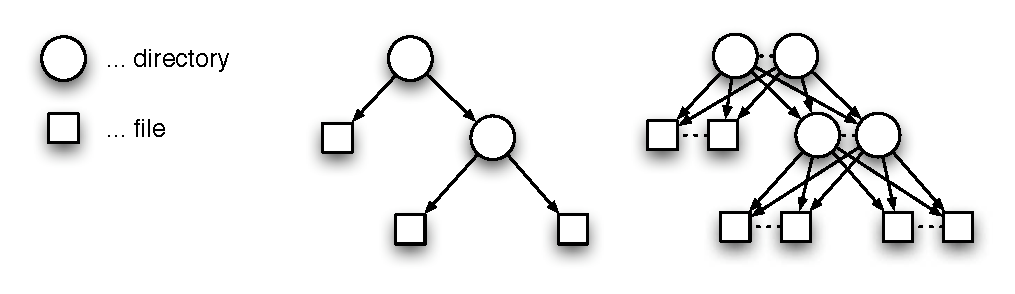
\includegraphics[scale=0.9]{figures/eps/fileSystem.eps}
\caption{
A comparison of a standard file system (left), and the proposed redundant file system (right). Parent-child relationships are indicated using arrows, clone relationships are indicated using dotted lines.
}
\end{figure}

We can summarize the above: \emph{a clone of a resource may be recovered if there exists a clone that is referenced by a valid clone of the parent}. Note that this (recursive) criterion contains no information regarding the location of either the resource's clone or the parent's clone, implying that \emph{if for each resource there exists at least one readable, valid clone, referenced by a readable, valid clone of the corresponding parent, the whole tree of resources may be recovered, if a valid clone of \textbf{the root resource} is available}. We call such a system a\label{typeOne} \textbf{Type I recoverable system}. The current prototype of the angel-application is such a system.

\begin{figure}[ht!]
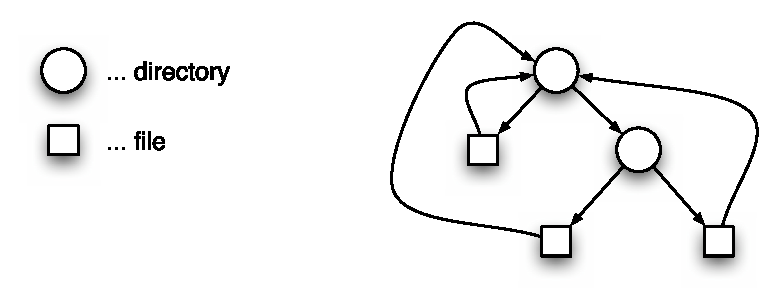
\includegraphics[scale=0.9]{figures/eps/fullyConnected.eps}
\caption{
Illustration of a fully connected resource graph (clone relationships have been left out for clarity). All file-type resources (previously leaf nodes) reference the root resource. Every resource may be reached from every other resource by following a sequence of arrows.
}
\end{figure}

 The last property implies that the root resource has no resources pointing to it -- maintaining a valid clone thereof is consequently somewhat unpleasant, though the task is in principle sufficiently small to be doable by hand. One practical \emph{ad hoc} solution to this problem, used in the current prototype, is that root resources (but not necessarily their child resources) are published in a central registry (to be provided and maintained by \emph{e.g.} MISSION ETERNITY). 

Another way to address this, is to note that the links used here are defined entirely in terms of the respective metadata of the parent and child resources, and it is therefore possible to construct circular structures. In particular, any resource may in principle link to the root resource (become a parent of the root resource). For example, we might require that all file resources (\emph{i.e.} leaf nodes) contain a link to the root resource. In that case, the link graph becomes \emph{fully connected}, \emph{i.e.} every resource is reachable from every other resource, and we may restate the above requirement on the recoverability of the resource graph as follows: \emph{if for each resource there exists at least one readable, valid clone, referenced by a readable, valid clone of the corresponding parent, the whole tree of resources may be recovered, if a valid clone of \textbf{any resource} is available}. We call such a system a\label{typeTwo} \textbf{Type II recoverable system}. Even in this case, it may nevertheless be advisable to publish a resource in a remote registry such as used for Type I systems.

A second particular property of the link structure is that there exist no \emph{a priori} constraints on the location and ownership of the parent and child resources. \emph{I. e.} a resource may link to any other resource \emph{independent of where it is physically located, or who it belongs to}. In other words, the system is \emph{composable} in the sense that individual resource networks can be combined to form larger networks. This is strictly analogous to the semantics of the Unix \texttt{mount} command. 

The above suggests a straightforward implementation of the central registry of root resources mentioned in this section -- the root resources are ``mounted'' on a reasonably persistent resource graph such as the one maintained by MISSION ETERNITY. Again, cyclic mounts are in principle possible (though care must be taken in the replication process). The act of publishing root resources can therefore also be expressed as a cyclic mechanism. For example, one could set up two networks $A$ and $B$, where network $A$ mounts the root resource of network $B$ and $B$ mounts the root resource of network $A$. This is analogous to the way cycle closures are obtained in Type II systems, which will only fail if many components fail at the same time.


\begin{figure}[ht!]
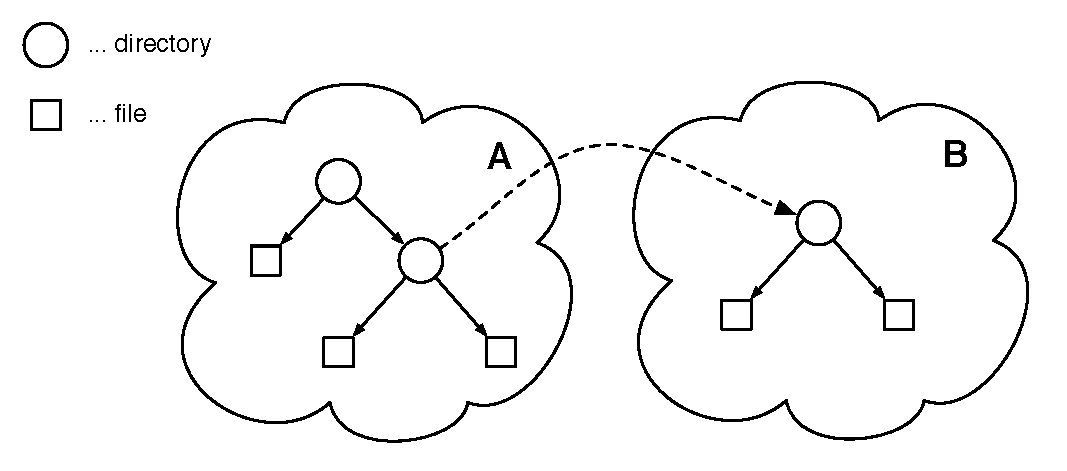
\includegraphics[scale=0.9]{figures/eps/mount.eps}
\caption{
A a resource in network \textbf{A} references the root resource of another network \textbf{B} (dashed arrow). Clone relationships have been left out for clarity. While in general, the two networks will be associated with different physical locations and belong to different users, the semantics of the link between the two networks are identical to the ones of intra-network links. 
}
\end{figure}

\subsection{Structure of a Resource}
\label{resource-structure}
We can now proceed to define the resource data structure as used in the angel-application. A resource consists of content and ``metadata''. If the resource is a ``file-type'' resource, the content is the file content as known from conventional filesystems. If the resource is a ``directory-type'' resource, the content is a piece of data identifying the resource as a directory (\emph{e.g.} the string ``directory''). Using an \emph{ad hoc} specification language, we write this as
\begin{verbatim}
resource := {content, metadata}
\end{verbatim}
The data fields associated with the resource can be either signed or unsigned, in order to do that, we require the existence of a ``public key'' metadata field specifying the owner. We require the existence of a metadata field consisting of the signature of the union of all signed metadata fields and the resource content. 
\begin{verbatim}
resource-owner := public-key
resource-signed-data := {resource-content, resource-signed-metadata}
resource-signature := signature(resource-owner, resource-signed-data)
\end{verbatim}
where the signed meta data fields for a resource are
\begin{verbatim}
resource-signed-metadata := {resource-identifier, resource-owner, 
                             resource-revision, resource-children, resource-encrypted}
\end{verbatim} \label{revision}
Metadata fields corresponding to partial signatures or intermediary checksums may be introduced (\emph{e.g.} for performance or simplicity reasons), as long as a checksum of the \texttt{resource-signed-data} is produced which cannot be produced without the secret key corresponding to \texttt{resource-owner}.
\texttt{resource-children} specify zero or more child resources
\begin{verbatim}
resource-children := resource-child*
resource-child := {child-identifier, child-owner}
\end{verbatim}
\texttt{child-identifier} is the identifier of the child resource, and \texttt{child-owner }is the public key (or a checksum thereof) of the child resource. \texttt{resource-id}, and \texttt{resource-revision} (for reasons we will explore in the following sections) are a union of a file path with a date, and a natural number ($\in \mathbb N_0$), respectively:
\begin{verbatim}
resource-id := {path, date}
resource-revision := natural-number
\end{verbatim} 
\texttt{resource-encrypted} is a boolean flag indicating whether the resource contents are encrypted
\begin{verbatim}
resource-encrypted := 0 | 1
\end{verbatim}
For reproducibility reasons, we suggest that the union operation used here be implemented as the result of a concatenation of UTF-8 string (XML) representations of the respective union members in the order presented here. When a resource is replicated inside the angel-application, the \texttt{resource-signed-data} must be completely replicated, otherwise the resulting clone is invalid. This latter property implies that resource replication is a transactional process -- it either succeeds completely, or results in a partial replication, which can be identified and discarded. \label{transaction}

Resources are additionally associated with unsigned fields. Unsigned fields may be freely introduced for configuration purposes, such as optimization of the graph traversal process. In particular, every resource is associated with a list of clones, and a list of clones for each of its children:
\begin{verbatim}
resource-clones := clone*
child-clones := clone*
clone := URL
\end{verbatim}
For simplicity reasons, the current prototype of the angel-application assumes that the \texttt{child-clones} may be inferred from the \texttt{resource-clones}, \emph{i.e.} assumes that if a remote clone exists for a local clone, then for a local child clone of the resource a remote child clone may be found for the remote clone.

\subsection{Traversing and Inspecting the Resource Graph}
\label{traverse}
We will first consider a \textbf{Type I} recoverable system (see section \ref{typeOne}), where we additionally impose that every resource has exactly one parent resource, or none, if it is the root resource, \emph{i.e.} the resource graph is a tree. This somewhat limits the kinds of available network topologies that the system supports, but it becomes easy to write an efficient, exhaustive graph-traversal algorithm, \emph{i.e.} an algorithm that visits every node exactly once. The current prototype of the angel-application requires this graph structure, and employs a depth-first tree traversal algorithm:
\begin{verbatim}
def graphWalker(node, getChildren, toEvaluate, backPack = None):
    """
    A generator that (lazily, recursively) applies an operation to a 
    directed graph structure.
    
    @param node the graph node where we start
    
    @param getChildren a callable f such that f(node) returns 
                       the child nodes of node
                       
    @param toEvaluate a callable g such that the result rr
                      for a node is rr = g(node, backPack)[0]
    
    @param backPack a partial result that is carried along and may 
                    change as the graph is traversed. 
                    g(node, backPack)[1] is passed on to the child nodes.
                    
    @returns an iterator over the results of applying toEvaluate to every 
             node in the tree
    """
    rr = toEvaluate(node, backPack)
    yield rr[0]
    for child in getChildren(node):
        for result in graphWalker(child, getChildren, toEvaluate, rr[1]):
            yield result
\end{verbatim}
where we use \texttt{backPack} to implement an optional maximum recursion depth. \texttt{getChildren} returns the URL's of the resource's \texttt{resource-children} (if any), and \texttt{toEvaluate} may be written as:
\begin{verbatim}
def toEvaluate(resource, depth = 0):

    if depth == 0: raise StopIteration
    
    goodClones, badClones, unreachableClones = completeCloneList(
        resource.startingClones(), 
        resource.publicKey(), 
        resource.ID())
    
    if goodClones == []: raise StopIteration

    resource.maintain(goodClones)
   
    goodClones += broadcastUpdate(goodClones, badClones)
    broadcastClones(goodClones)
    
    resource.setClones(goodClones, unreachableClones)

    broadCastClones(goodClones)
    storeClones(af, goodClones, unreachableClones)
\end{verbatim}
Here, \texttt{startingClones} is a function that generates a first guess for the set of clones of the resource. \texttt{completeCloneList} is a function that takes such an intitial guess, and (given a resource identifier and key), validates these clones. From those clones that are found to be valid, the respective clone lists are requested, and the procedure is repeated. At the end of the procedure, we have generated three lists of clones: (i) clones that are reachable and have been found to be valid, (ii) clones that are reachable and have been found to be invalid, and (iii) clones that are not reachable. Together these three lists contain all known (or rather, guessed) clones, of all reachable clones. If no valid clones are found, this branch of the resource tree is ignored in this iteration. \texttt{maintain} is a function that takes a list of valid clones and compares one of them to the local clone, if the local clone is found to be invalid, it is replicated from the list of good clones. Once the local clone is valid, we can attempt to update the bad clones from the local clone. This step is in principle optional, and requires a mechanism for controlled write access from remote peers, which is described in section \ref{access}. \texttt{broadCastClones} broadcasts the newly obtained list of good clones to all good clones.

In this approach, the graph is assumed to be tree-like, \emph{i.e.} ring structures are not accounted for except for the (optional) use of a recursion-depth limit. This seems sufficient for \textbf{Type I} systems, and especially so for such systems that close model a file-system tree. However, ring structures are pervasive in \textbf{Type II} systems. Most of these ring structures involve a (arbitrarily chosen) root node, in which case an \emph{ad hoc} approach involving recursion termination upon traversal of the root node seems appropriate. The generalization and optimization of the graph traversal to better account for cyclic structures and local optimizations will be the scope of future work.

\section{Living in a Dynamic Network}
\label{dynamic}

The previous section has dealt with a static hierarchy of resources, and did not directly tackle the issues of data migration and modification. In other words, it was not discussed what happens if a user decides to join or leave a contract, when machines hosting an angel-app node come online or go offline, or, most importantly, how a resource is supposed to be modified, added, or deleted. When postulating support for the above operations, we must first acknowledge that it can not be guaranteed that a node exists, that a message can be sent to it, or that it will react to a message in a predictable way. In particular, it must be assumed that some nodes may in fact be hostile, implying that for a message to be accepted, it must pass certain authorization criteria. The system must be \emph{Byzantine fault tolerant}.

To discuss these issues, let us once again start with a few definitions. A \emph{user} is the owner of zero or more resources, \emph{i.e.} she holds one or more secret keys. A \emph{node} is an instance of the angel-app that provides a query interface to a collection of resources stored ``on'' the node. One user is the \emph{peer} of another user. And one node is the peer of another node. The angel-app must then be organized in such a way that peers are not required to trust each other. However, in order to take advantage of peer-to-peer networking, it must also be organized in such a way that peers \emph{may} trust each other user where appropriate.

The overall approach is then the following: \emph{a user must be able (though not necessarily forced) to set up a node in such a way that in the limit of the absence of suitable peers, or catastrophic failure of many or even all of them (breakdown of the electronic or social network) the angel-app will continue to operate in much the same way as a normal file system, though without the benefits of replication and redundancy}.

The fulfillment of the above requirement is verified from the contents of Section \ref{backup}:
\begin{enumerate} 
\item In the absence of remote clones, and assuming that for each resource there exists a local clone, the angel-app directly models a local file system. Such a system is clearly byzantine fault tolerant (at least in a single-user environment).
\item Clone replication is entirely based on \emph{verifyable} claims made by the peer node. A system such as the above extended with a replication mechanism is therefore also byzantine fault tolerant.
\item We believe that the following section describes a byzantine fault tolerant approach to propagating resource modifications and updates and we therefore claim that the overall system is also byzantine fault tolerant. 
\end{enumerate}

\subsection{Adding, Modifying and Removing Resources}

We have so far considered individual resources to be static, immutable entities. In order to deal with mutability, let's start out by noting that there are essentially two types of mutable graph structures. In structures involving destructive updates, the original structure is \emph{replaced} by the new structure, and the original structure is therefore \emph{permanently lost}. Common file systems are such structures. Alternatively, copy-on-write mechanisms may be used, \emph{i.e.} if a node is updated, a copy of the old node is retained, and is in general recoverable, but the user is presented with the modified graph. In this context, the latter approach is used \emph{e.g.} in the Google File System\cite{gfs}, or in common version control systems such as Subversion\cite{svn} or darcs\cite{darcs}. This approach has obvious advantages in terms of longevity -- information is more difficult to destroy using system-internal mechanisms. When coupled to an approach where data is difficult to destroy via system-external processes (\emph{i.e.} an approach such as the angel-app or the Google File System), the resulting data structures can obviously exhibit great resilience to data loss in general. On the other hand, if a model allowing destructive updates is used, catastrophic data loss may still occur due to authorized user input, even if all possible causes of data loss due to external processes such as media failure can be ruled out.

Still, the angel-app for now implements the notion of destructive updates, the reasons being that
\begin{itemize}
\item we aim to closely model standard file system semantics, which typically allow for destructive updates;
\item it seems straightforward to meaningfully implement a copy-on-write mechanism (possibly as an optional extension) in a system that allows destructive updates, while the reverse is likely not the case.
\end{itemize}

We have briefly introduced the notion of a revision number (a signed metadata field) in Section \ref{revision}. In a fully connected network of nodes where all nodes are permanently online, the semantics of modifying a resource then become rather simple: if a user has access to the secret key of the resource she is free to modify the resource data, and generate and store the required resources. All we then need to do is to replace the clones of the old resource by clones of the new resource. We can accomplish that by incrementing the revision number upon modification and requiring that in the clone maintenance process (Section \ref{traverse}), a valid local clone is replaced by a valid remote clone if the revision number of the remote clone is higher than that of the local clone. Complying nodes will therefore replicate the most current version of a resource, while the corresponding clones residing on ``evil'' nodes will be ignored from this point on.

To add a resource, we 
\begin{enumerate}
\item add a  \texttt{resource-child} reference (see Section \ref{resource-structure}) to the resource's parent, implying that a user can only add resources in directories she has the secret key of, and 
\item increase the parent's revision number.
\end{enumerate}
The modified parent and the resource itself will then automatically be replicated to suitable clones (Section \ref{traverse}). Similarly, deletion operations may be implemented by removing the \texttt{resource-child}  reference to the resource from the resource's parent, and requiring that upon update of the parent all local child resources are removed that are not referenced by the parent.

\subsection{Multiple Nodes and Multiple Users}
\label{multiple}
Let us first consider what happens when a node of the angel-app network comes online, either after it has been newly initialized, or after it has been intermittently offline for some time for another reason. In both cases, it will start by obtaining a root resource of some sort, and then proceed to replicate the rest of the resource graph starting from this root resource. Due to the transactional nature of clone replication (see Section \ref{transaction}), and the robustness properties of the graph replication process (see Section \ref{typeOne}) this will eventually succeed \emph{exactly if there exists no unreachable, modified clone  with a revision number smaller or equal to the current revision number of the resource}.

To illustrate the above, consider the following scenario: let Alice and Bob be users running different nodes, but with access to the same secret key. Let there be no communication channel between them (\emph{i.e.} at least one of them is ``offline''). Let both of them perform modifications of the same resource. When Alice and Bob re-establish their communication channel, the modifications of (at least) Alice or of Bob will get lost if the corresponding revision numbers are not the same. If the corresponding revision numbers are the same, the behavior of the graph inspection will be undefined. 

We therefore require that additionally at least one of the following constraints holds:
\begin{itemize}
\item for every resource, there exists just one node with access to the corresponding secret key;
\item if multiple nodes exist that have access to the secret key of a given resource, modifications of this resource are only allowed if a suitable locking mechanism exists to prevent conflicting modifications. 
\end{itemize}
The implementation (and implementability) of such a locking mechanism obviously greatly depends on the usage patterns, network topology and the local structure of the resource graph, and a specification for the angel-app has therefore so far not been attempted. However, the following observation should serve as a significant simplification when attempting such an implementation: nodes that share a secret key may generally be assumed to be able to trust each other.

The former approach (currently taken, required, but not enforced by the angel-app) has the additional property that \texttt{resource-id}'s can be easily generated: if the creation of a resource on a given node corresponds to the creation of an actual file on the node's file system (\emph{i.e.} is associated with a specific path), and the corresponding file can only be created on this specific node (since secret keys are not shared), the combination of creation time, creation path, and public key is guaranteed to form a globally unique identifier, as required by Section \ref{maintain}.

\section{Practical Implementation Considerations}

\subsection{Transparent and Safe Access}
\label{access}

The previous sections operated in an idealized environment, in which the user could be implicitly burdened with the task of keeping track of keys,  and of the encryption and signing of data. This is obviously not acceptable for a real-world system that aims to be user-friendly. To remove this dependency and still provide file-system semantics for day-to-day operations, we have chosen to hide the resource graph behind a standard network file system protocol (where we have chosen WebDAV for portability and simplicity). The advantages of this approach are:
\begin{itemize}
\item Day-to-day file system operations (opening, modifying, closing a file) are seamlessly supported (including all external tools such as file search mechanisms) on operating systems that support the corresponding network file system protocol.
\item The task of encrypting, decrypting and signing data can be transparently handled by a locally running server of that file system protocol;
\item Access to resources that are not locally stored can be transparently managed, optional caching mechanisms are easily implemented.
\item The implementation of the file system protocol may be used as a messaging protocol between angel-app nodes, reducing overall redundancy in the code.
\end{itemize} 

The resulting proposed structure of an angel-app node is displayed in Figure \ref{webdav}: Basic file system operations are available to the user via standard file managers, while bookkeeping and encryption are transparently handled by a locally running network file system server. Administration tasks which can not be expressed as file system operations may be performed through a custom configuration interface. The implementation of the file system protocol is also used for inter-node messaging.

\begin{figure}[ht!]
\begin{center}
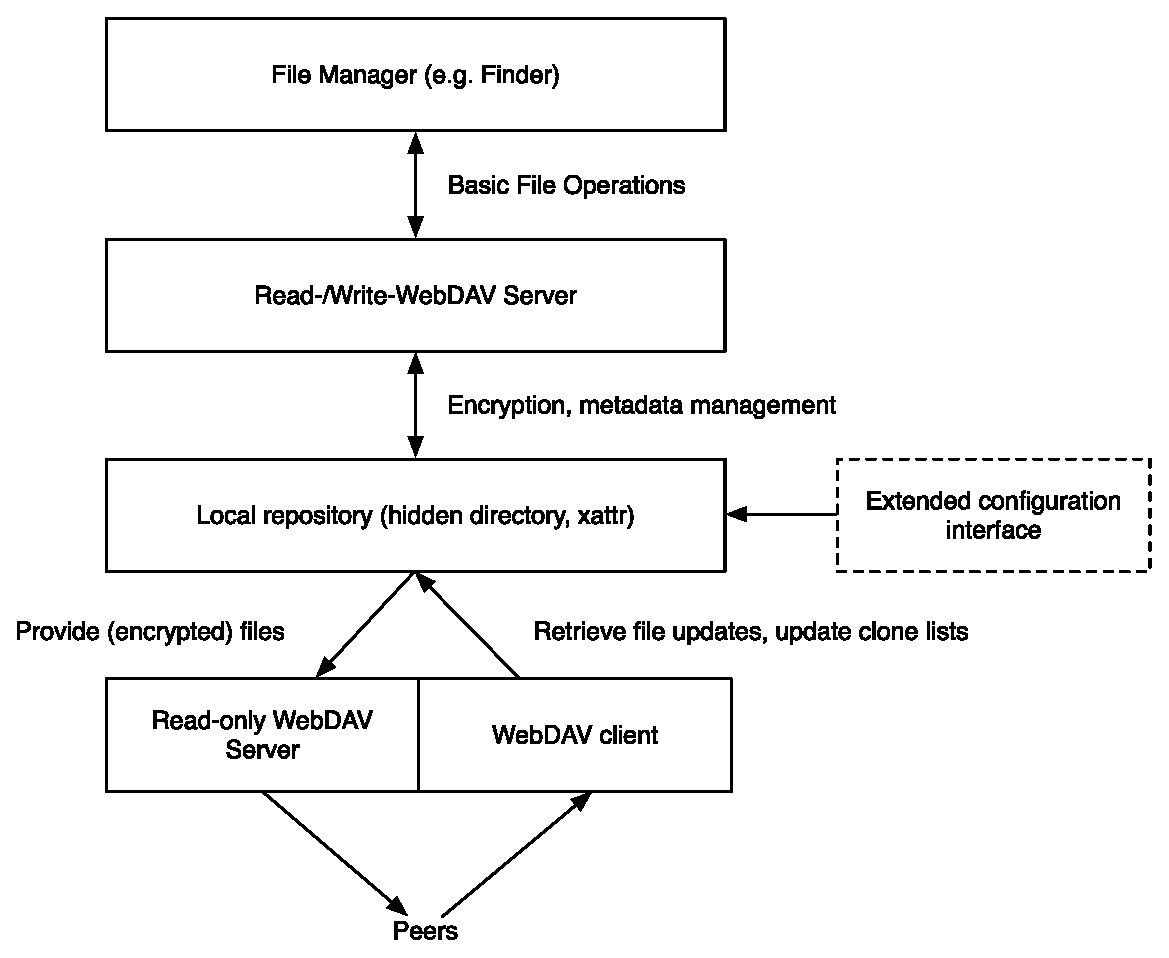
\includegraphics[scale=0.7]{figures/eps/webdav.eps}
\end{center}
\caption{Layout of an angel-app node. Basic file system operations are available to the user via standard file managers, while bookkeeping and encryption are transparently handled by a locally running network file system server. Administration tasks which can not be expressed as file system operations may be performed through a custom configuration interface. The implementation of the file system protocol is also used for inter-node messaging.}
\label{webdav}
\end{figure}

It seems worthwhile to note that the angel-app can thus be cleanly separated into a number of different processes. An ``internal'' server (with access to the user's secret key, and typically listening only for connections from the machine the node is hosted on) and a (also locally running) configuration interface handle authenticated user input. The communication channels that are exposed to the outside network have read/write access to the locally stored resources, but no signing capability. Unauthorized access to the secret keys is therefore easy to avoid.

\subsection{Peer Visibility}

The wide-spread use of network-address-translation (NAT) and firewalling techniques make the deployment of the angel-app on wide area networks (WAN's) somewhat difficult. Nodes running the angel-app may be unable to send messages to each other, even if they are in principle ``online''. A definitive solution for this problem should require the use of one or more of the following, and is the scope of future work:
\begin{itemize}
\item firewall hole-punching techniques such as UDP hole-punching;
\item dynamic firewall configuration via mechanisms such as UPnP;
\item request relaying via ``super-nodes''.
\end{itemize}
The current (temporary) solution to this problem can be interpreted as an \emph{ad hoc} implementation of the latter approach. It makes use of the fact that (in the absence of a mechanism to enforce distributed resource locks) no hard limits exist on the time that message-passing may take. Namely in contrast to \emph{e.g.} instant-messaging systems, messages in the context of the angel-app consist entirely of replication requests, which may take an essentially arbitrary amount of time (days or more). For the replication of a clone from a node $A$ to a node $B$, with nodes $A$ and $B$ being unable to communicate directly, it is therefore (more than) sufficient to require that a node $C$ exists, such that the clone can be replicated to $C$ and that $C$ is visible by both $A$ and $B$. This in turn is requires that a ``push'' mechanism exists, by which $A$ can initiate the replication of the resource to $C$. Once the this replication step is completed, the clone is visible from $B$.


\section{Possible Future Developments}

\begin{itemize}
\item Revision Control:
Maintain history of individual resources. With an undo function. Since changes are a per-resource property, this seems straightforward to do.

\item Load-Balanced Distribution:
If a resource is stored on multiple nodes, we can use the bandwidth of all nodes to distribute the resource bittorrent-style.

\item Complex Authentication Schemes:
What if users running different nodes want to modify a given resource? So far, we imposed that they can not both have access to the secret key -- set one node up as the master node and proxy requests through that?

\item Shared Workspaces:
Once we have the above, we can implement shared workspaces -- multiple users can safely operate on the same data, and have (at least) read-only access to that data, \emph{even if they are offline}.
\end{itemize}

\end{mainmatter}

\begin{thebibliography}{99}
\bibitem{oceanstore} OceanStore: An Architecture for Global-Scale Persistent Storage, John Kubiatowicz, David Bindel, Yan Chen, Steven Czerwinski, Patrick Eaton, Dennis Geels, Ramakrishna Gummadi, Sean Rhea, Hakim Weatherspoon, Westley Weimer, Chris Wells, and Ben Zhao. Proceedings of the Ninth International Conference on Architectural Support for Programming Languages and Operating Systems (ASPLOS 2000), November 2000.
\bibitem{pastiche} Pastiche: Making Backup Cheap and Easy. Landon P. Cox, Christopher D. Murray, and Brian D. Noble.  In the Fifth Symposium on Operating Systems Design and Implementation. Boston, MA, December 2002.
\bibitem{keso} Keso, A scalable, reliable and secure read/write peer-to-peer file system, Mattias Amnefelt and
Johanna Svenningsson, 2006.
\bibitem{mstore} MyriadStore: APeer-to-PeerBackupSystem, Birgir Stefansson and Antonios Thodis, 2006. 
\bibitem{freenet} Protecting Free Expression Online with Freenet. Ian Clarke, Scott G.Miller, Theodore W.Hong, Oskar Sandberg, and Brandon Wiley. IEEE internetcomputing,  2002.
\bibitem{gfs} The Google File System, Sanjay Ghemawat, Howard Gobioff, and Shun-Tak Leung, available online.
\bibitem{svn} The Subversion Version Control System, available at online.
\bibitem{darcs} The Darcs Revision Control System, available online.
\end{thebibliography}

\end{document}